\chapter{Baseline Compensation System}
Baseline compensation system is a one of the active vibration isolation system for GW detector's arm cavity. 

In the section \cref{sec:51}, the passive viblation isolation is described. After that, two type of active vibration isolation system are described in the section \cref{sec:52} and \cref{sec:53}. In the section \cref{sec:54}, the baseline compensation system is described.

\section{Basics in Seismic Isolation}\label{sec:51}
Essentialy, the vibration isolation system has a pendulum to attenuate the seismicnoise passively. For further the isolation performance, the pendulum have developed as a longer and multi-stage pendulum.

\subsection{Single Pendulum}
For simple example, as shown in left figure in Figure(\ref{img:img501}), consider a one-dimentional harmonic oscillator consisting of a spring with a spring constant $k$ and mass $M$. The displacement of the suspension point and the mass are $x_0$ and $x$, respectively. Because the equation of the motion is written as
\begin{eqnarray} \label{eq:eq501}
  M\ddot{x} = -k(x-x_0),
\end{eqnarray}
the frequency transfer function from the displacement of the suspension point to the mass displacement $H(f)$ is given by the Fourier transform from the equation and represented as
\begin{eqnarray} \label{eq:eq502}
  H(f) \equiv \frac{1}{1-(f/f_0)^2},
\end{eqnarray}
where $f_0 = (k/M)^{1/2}$ is the resonant angular frequency of the oscillator.

According to Eq.(\ref{eq:eq502}), the amplitude of $H(f)$ is unity below the resonant frequency, the amplitude is approximately propotional to $(f/f_0)^{-2}$ above resonance frequency. The bode plot of $H(f)$ with various resonance frequencies are plotted in right figure in Figure \ref{img:img501} . One finds that it is better to make a low-resonance frequency oscillator in order to attenuate the seismic noise broadly. 

\begin{figure}[h]
  \begin{center}   
    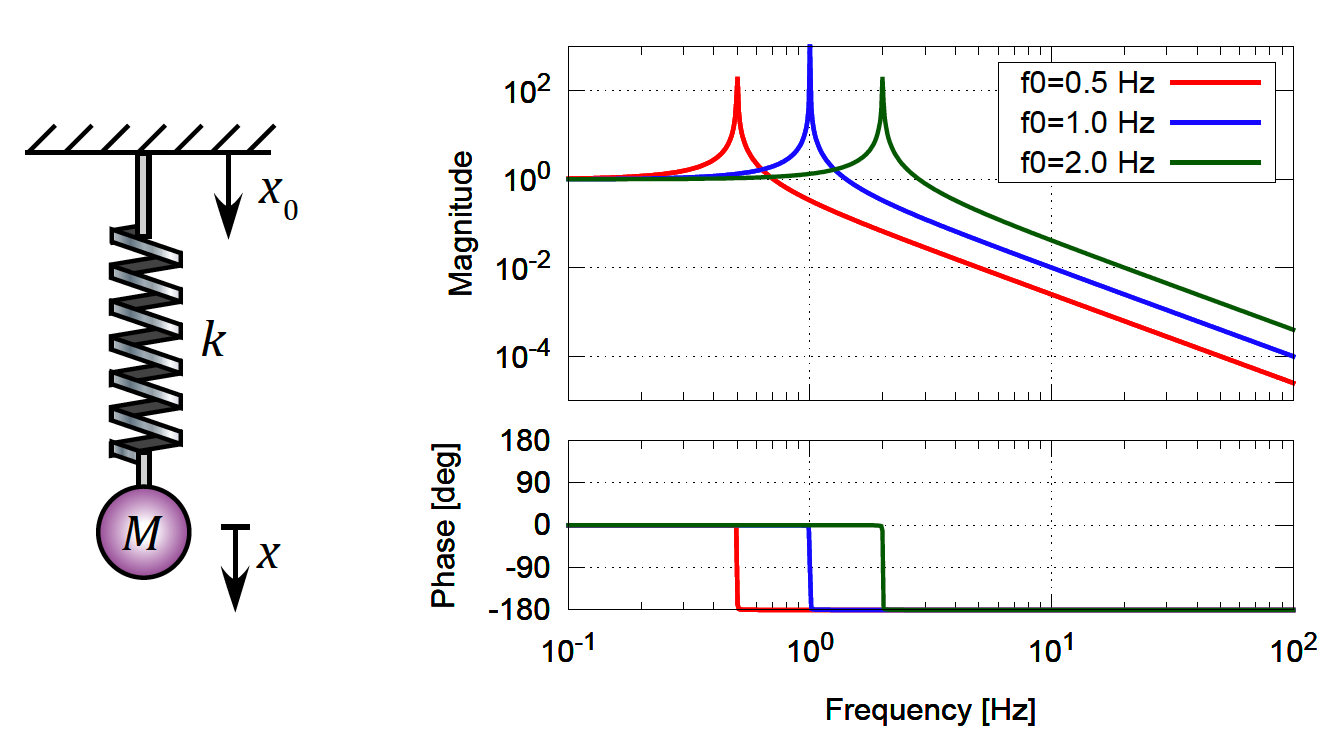
\includegraphics[width=11cm,height=6cm]{./img_chap5/img501.png}
    \caption{Single pendulum as a mechanical filter and its transfer function with various resonant frequencies. This figure is cited from Figure(2.3) in \cite{sekiguchi2016astudy}.} \label{img:img501}
  \end{center}
\end{figure}

\subsection{Multi-stage Pendulum}
In order to increase the order of the seismic isolation, multi-stage pendulum is effective. In case of an N-stage pendulum, the transfer function from the ground to the suspended mass is propotional to $f^{-2N}$ above the resonance frequrncy of the pendulum as shown in Figure \ref{img:img502}. 
\begin{figure}[h]
  \begin{center}   
    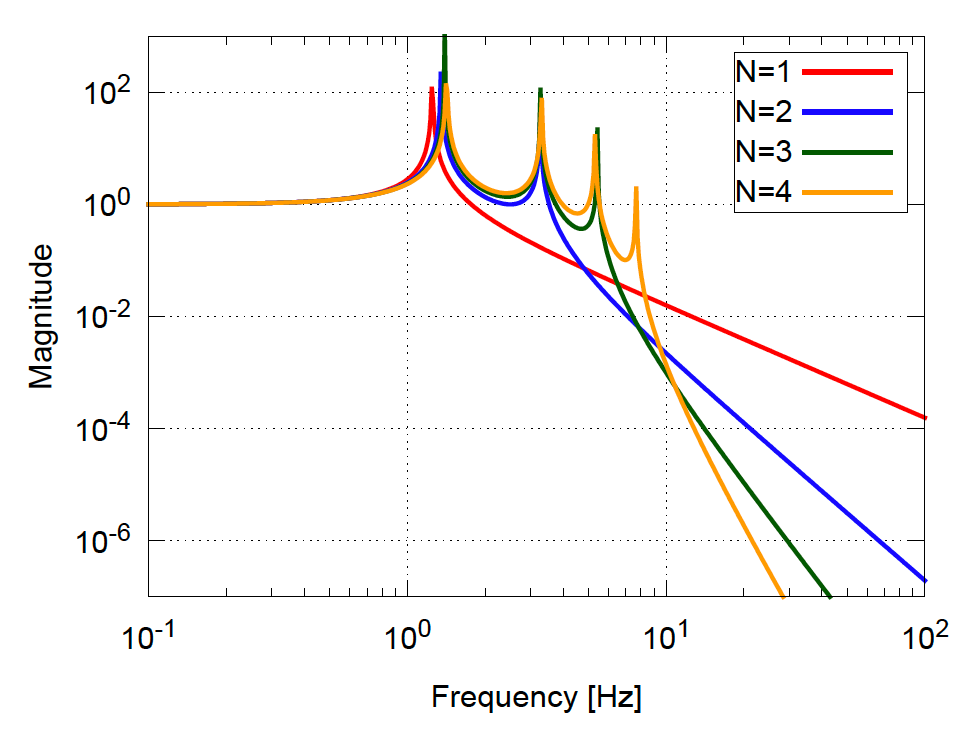
\includegraphics[width=10cm,height=7cm]{./img_chap5/img502.png}
    \caption{The amplitude of the transfer function of the N-stage pendulum. This figure is cited from Figure 2.4 in \cite{sekiguchi2016astudy}.} \label{img:img502}
  \end{center}
\end{figure}


\section{Active Inertial Seismic Isolation}\label{sec:512}
\begin{figure}[h]
  \begin{center}
    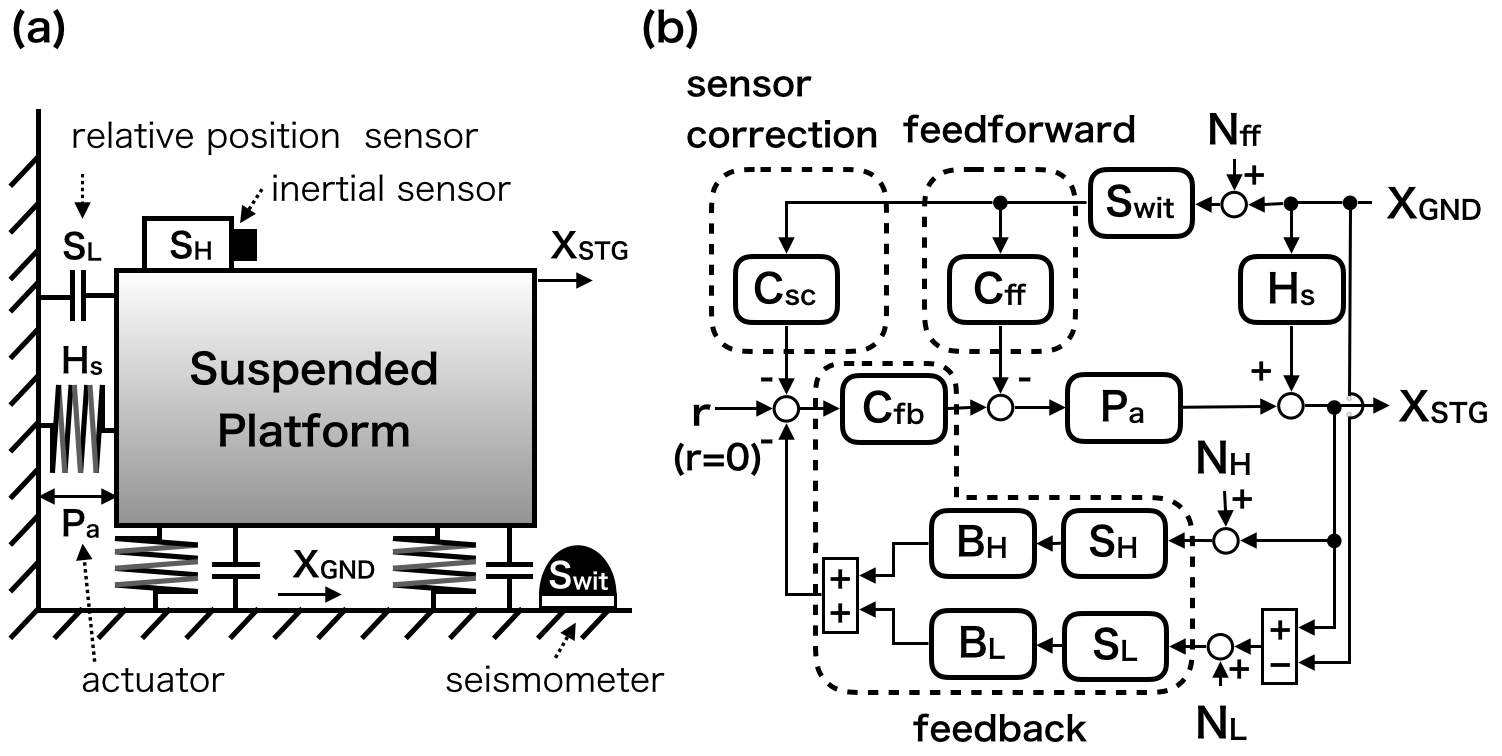
\includegraphics[width=13.5cm]{./img_chap5/img503.png}
    \caption{{\bf(a)} Schematic drawing of an active seismic isolation system for platform. {\bf(b)} Block diagram of the active control scheme.} \label{img:img503}
  \end{center}
\end{figure}
The passive vibration isolation cannot reduce the seismic noise below its pendulum's eigenfrequency. To attenuate the lower-frequency seismic noise, the active vibration isolation system using a seismometer \cite{matichard2015seismic}.

The active isolation system is shown in Figure \ref{img:img503}(a). A platform is suspended from the ground with transmisivity $H_{\mathrm{s}}$. This platfrom is fed back both signal of a inertial sensor with calibration factor $S_{\mathrm{H}}$ and signal of a relative position sensor with calibration factor $S_{\mathrm{L}}$, to the platform using actuator with actuator efficiency $P_{\mathrm{a}}$. This feedback control actively decouple the platform from the seismic disturbance from $0.1\,\mathrm{Hz}$ to a few Hz. Moreover, the platform is controled with feedforward using a seismometer with calibration factor $S_{\mathrm{wit}}$ installed on the local ground. 

As shown in Figure \ref{img:img503}(b), the active vibration system is integrated with a feedback control, sensor correction contorl, and feedforward control. These control schemes are described below.

\subsection{Sensor Blending Technique}
\begin{figure}[h]
  \begin{center}   
    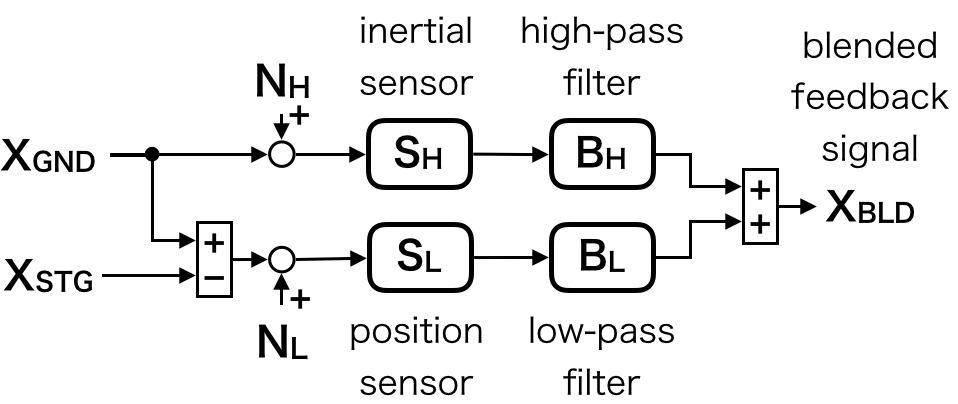
\includegraphics[width=10cm]{./img_chap5/img507.png}
    \caption{Sensor Blending.} \label{img:img507}
  \end{center}
\end{figure}

The purpose of the active inertial seismic isolation is to reduce the stage motion against the inertial frame. Thus, we use the feedback control using a inertial sensor. However, because the noise level of the inertial sensor is worse in low-frequency regison, the feedback system cannot use the inertial sensor in this region. Nevertheless, to control the DC position of the stage. In this situation, the sensor blending technique is commonly used in the active viblation system.

As shown in Figure \ref{img:img507}, the feedback signal is belended by singals of the inertial and position sensors. The inertial sensor output is filterd with high-pass filter $B_{\mathrm{H}}$ because noise of the sensor is worse in low-frequency region. On the other hand, the position sensor is filterd with a filter $B_{\mathrm{L}}$ so that
\begin{eqnarray}
  B_{\mathrm{H}}S_{\mathrm{H}} + B_{\mathrm{L}}S_{\mathrm{L}} = 1,   \label{eq:eq506}
\end{eqnarray}


In the case of using the blended feedback signal, the displacement of the platform stage. The displacement of the stage is given by
\begin{eqnarray}
  X_{\mathrm{STG}} = \frac{G}{1+G}LX_{\mathrm{GND}} + \frac{1}{1+G}H_{\mathrm{s}}X_{\mathrm{GND}} + \frac{G}{1+G}\left(HN_{H}+LN_{L}\right),   \label{eq:eq510}
\end{eqnarray}
where $X_{\mathrm{STG}},\,X_{\mathrm{GND}},\,N_{\mathrm{H}},$ and $N_{\mathrm{H}}$ are the displacement of the stage and the ground motions, and the noise of the inertial sensor and the position sensor, respectively. Moreover $G=C_{\mathrm{fb}}P_{\mathrm{a}}$ is the loop gain, and the multiples of the comprimentary filters and each sensor responses are defined as $L=B_{\mathrm{H}}S_{\mathrm{H}}$ and $H=B_{\mathrm{L}}S_{\mathrm{L}}$, respectively. Here, if the feedback is work enough, thus the loog gain is large enough, the displacement of the stage is given as
\begin{eqnarray}
  \lim_{G\to\infty} X_{\mathrm{STG}} = LX_{\mathrm{GND}} + \left(HN_{H}+LN_{L}\right) \label{eq:eq510_a}
\end{eqnarray}

According to Eq.(\ref{eq:eq510_a}), to isolate the stage against the inertial frame, the active isolation system should design $L$ as small as possible, whereas the $H$ as the complementary filter of that must be large, which means that the inertial sensor noise introduce to the stage. Actually, the cutoff frequency of these filters are choosed at $100\,\mathrm{mHz}$ due to the inertial sensor noise, and the system cannot isolate the seismic noise below this frequency. In other words, although the active vibration syste using the inertial sensor can design the response from the ground to the stage by filter $L$, the system performance is limited by the inertial noise in low-frequency region.

\subsection{Sensor Correction Technique} \label{sec:sec513}
\begin{figure}[h]
  \begin{center}   
    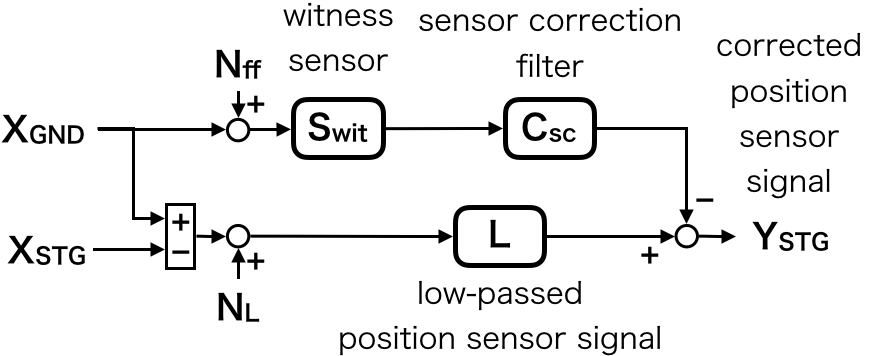
\includegraphics[width=10cm]{./img_chap5/img505.png}
    \caption{Sensor correction scheme.} \label{img:img505}
  \end{center}
\end{figure}
Sensor correction technique is a method to correct the posision sensor using the additional inertial sensor on the ground \cite{hua2005low}. As mentioned above, because of the insufficient noise of the inertial sensor on the stage, the blended feedback signal use had to use the position sensor in the low-frequency. This means that the stage motion is reduced to the local ground frame not inertial frame in this frequency region. Thus, the sensor correction remove the groung motion from the position sensor by using anothor seismometer on the ground that have better sensitivity than the inertial sensor on the stage. The corrected feedback signal can compensate the performance of the inertial sensor on the stage.

Consider the displacement of the vibration isolated stage utilizing sensor correction technique. As shown in Figure\ref{img:img503}, the correction signal from the seismometer signal is injected at the set-point through the control filter $C_{\mathrm{sc}}$ to remove the ground motion from the feedback signal using the position sensor. The displacement of the stage is given by 
\begin{eqnarray}\nonumber
  X_{\mathrm{STG}} &=&\frac{G}{1+G}L\left(1-C_{\mathrm{sc}}\frac{S_{\mathrm{wit}}}{L}\right) X_{\mathrm{GND}} + \frac{1}{1+G}H_{\mathrm{s}}X_{\mathrm{GND}}\\ 
  &+& \frac{G}{1+G}\left(HN_{H}+LN_{L}\right) + \frac{G}{1+G}C_{\mathrm{sc}}S_{\mathrm{wit}}N_{\mathrm{ff}} \label{eq:eq511}
\end{eqnarray}
Here, in the case that the loop gain is large enough, the stage motion is given by 
\begin{eqnarray}
  \lim_{G\to\infty} X_{\mathrm{STG}} = L\Delta_{\mathrm{sc}} X_{\mathrm{GND}} + \left(HN_{H}+LN_{L}\right) + {L}N_{\mathrm{ff}} \label{eq:eq513},
\end{eqnarray}
where 
\begin{eqnarray}
  \Delta_{\mathrm{sc}} \equiv \left(1-C_{\mathrm{sc}}\frac{S_{\mathrm{wit}}}{L}\right) \label{eq:eq512}
\end{eqnarray}
is the gain matching coeffient. By comparison with Eq.(\ref{eq:eq513}) and Eq.(\ref{eq:eq510_a}), the displacement of the stage can be reduced by the gain matching.

Although this gain maching factor can be zero when $C_{\mathrm{sc}}=B_{\mathrm{L}}(S_{\mathrm{wit}}/S_{\mathrm{L}})$, actually, the factor is limited by the caliblation errors of the witness sensor and the inertial sensor on the stage. At least, the error can not be less than 5\%, so it is difficult to achieve the vibration isolation ratio of 20 \cite{hua2005low}.

\subsection{Feedforward Technique}
\begin{figure}[h]
  \begin{center}   
    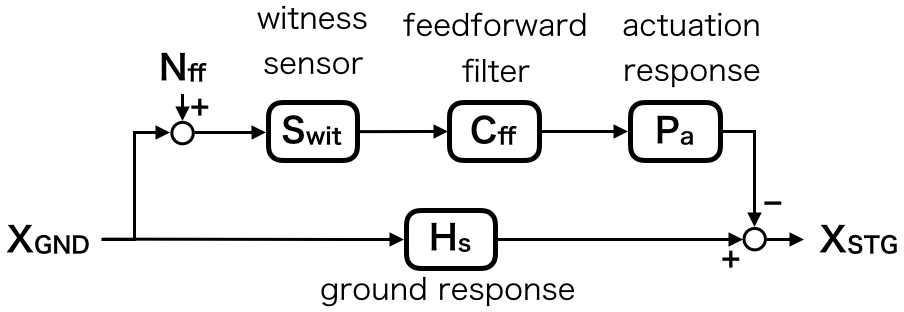
\includegraphics[width=10cm]{./img_chap5/img506.png}
    \caption{Feedforward scheme.} \label{img:img506}
  \end{center}
\end{figure}
Feedforward technique is similar to sensor correction, but this technique remove the motion caused by the ground motion directly. Figure\ref{img:img506} shows the block diagram of the feedfoward control. While the stage motion $X_{\mathrm{STG}}$ is disturbed by the ground motion $X_{\mathrm{GND}}$ through the mechanical response of the platform $H_{\mathrm{s}}$, the feedforward compensates the stage motion by subtracting the disturbance with the witness sensor (in this case, seismometer) signal. This feedforward control does not depend the feedback control unlike the sensor correction. In other words, the feedforward control works in the frequency region where the feedback loop gain is small, whereas the sensor correction works in the high loop gain region. Therefore, both feedforward and sensor correction technique is used to improve the vibration isolation system in all frequency region.


Finally, consider the control integrated with three techniques; sensor blending, sensor correction, and feedforward. In the case that the additional feedforward signal is injected at the error-point, as shown in Figure \ref{img:img503}, the displacement of the stage motion is given by
\begin{eqnarray}\nonumber
  X_{\mathrm{STG}} &=&\frac{G}{1+G}L\Delta_{\mathrm{sc}} X_{\mathrm{GND}} + \frac{1}{1+G} \Delta_{\mathrm{ff}} X_{\mathrm{GND}}\\ \nonumber
  &+& \frac{G}{1+G}\left(HN_{H}+LN_{L}\right) + \frac{G}{1+G}C_{\mathrm{sc}}S_{\mathrm{wit}}N_{\mathrm{ff}} \\ 
  &+& \frac{1}{1+G}P_{\mathrm{a}} C_{\mathrm{ff}}S_{\mathrm{wit}}N_{\mathrm{ff}} \label{eq:eq514}.
\end{eqnarray}
Here, 
\begin{eqnarray}
  \Delta_{\mathrm{ff}} \equiv \left(H_{\mathrm{s}}-P_{\mathrm{a}}C_{\mathrm{ff}}S_{\mathrm{wit}}\right) \label{eq:eq515}
\end{eqnarray}
is defined as the gain matching coefficient of the feedforward. One can find that, in  Eq.(\ref{eq:eq514}),  the first and second terms indicating the contribution from the ground motion can be reduced by the gain matching factors: $\Delta_{\mathrm{sc}}$ and $\Delta_{\mathrm{ff}}$. This reduction works independant from the feedback loop gain.

\subsection{Problem in Tilt-Horizontal Coupling}
The inertial sensors have problem in horizontal measurement in low-frequency due to a coupling from the tilting. This is called the tilt-horizontal coupling. Because of this coupling the feedback control using the inertial sensor cannot suppress the horizontal seismic motion aggressivly.

\subsubsection{Tilt-horizontal coupling}
\begin{figure}[h]
  \begin{center}   
    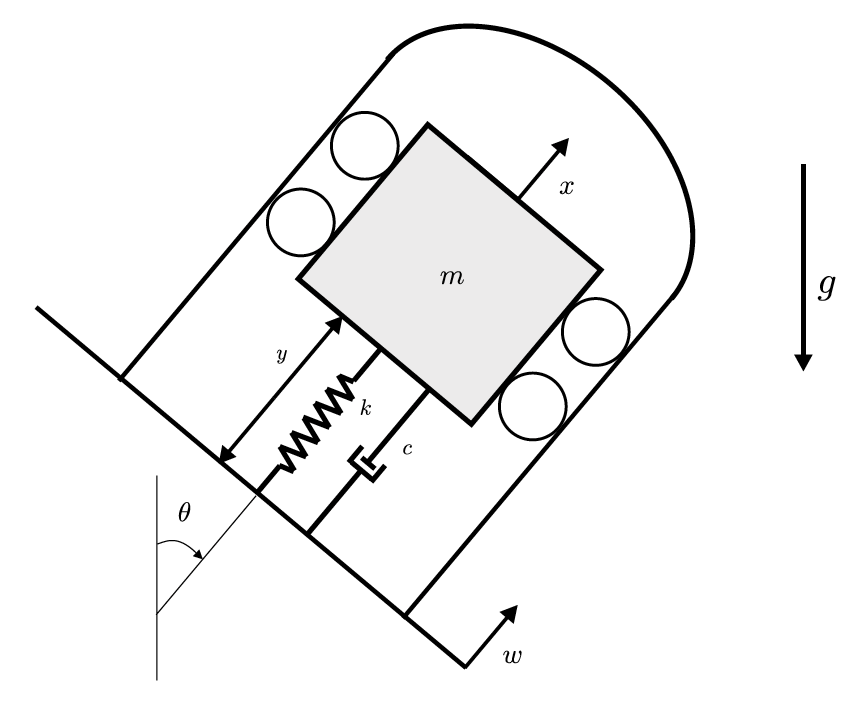
\includegraphics[width=8cm]{./img_chap5/img509.png}
    \caption{Tilted inertial sensor. Cited from Figure12 in \cite{collette2012inertial}} \label{img:img509}
  \end{center}
\end{figure}
 The inertial sensors cannot distinguish the horizontal or tilt motions of the ground because the inertial sensor measure the apparent force from the sensor frame. This coupling is known as the tilt-holizontal coupling and the response from each ground motion is given by \cite{collette2012inertial}
\begin{eqnarray}
  Y(s)=\frac{-m s^{2}}{m s^{2}+c s+k} \left[ W(s) + \frac{g \sin \left(\theta_{0}\right)}{s^2} \Theta(s) \right] \label{eq:eq515},
\end{eqnarray}
where $W(s),\,Y(s)$, and $\Theta(s)$ are, Laplace transformed, the displacement of the mechanical oscillator in the sensor, the relative displacement of the oscillator and the house enclosuring it, and the tilting angle of the house, respectively. Moreover, $m,\,c,\,k,\,g,$, and $\theta_0$ are the mass of the osclillator's proof mass, viscous damping coefficient, spring constant, and gravitational acceleration. According to Eq.(\ref{eq:eq515}), when 
\begin{eqnarray}
  f < \sqrt{\frac{g\sin(\theta_0)}{(2\pi)^2}}\ [\mathrm{Hz}]
  \label{eq:eq515}
\end{eqnarray}
the tilt motion tends to couple to the horizontal motion. For example, in the case of the maximum tilt coupling: $\theta_0=\pi/2$, the tilt motion contaminates the horizontal motion when $f<0.5\ [\mathrm{Hz}]$.

\subsubsection{Control strategy to avoid the problem}
As described above, the inertial sensor cannot be used for measuring the horizontal motion because of the inertial sensor behaving the tilt sensor. For the reason, the active inertial seismic isolation system in LIGO use the tilt sensor to remove the tilt components in the inertial sensor for avoiding the tilt-horizontal problem \cite{biscans2018optimization}.


\section{Active Baseline Seismic Isolation}
For laser interferometric gravitational-wave detector, the baseline length should be isolate from the seismic noise, whilie it is not necessary to isolate the individual stages to the inertial frame. For this reason, the active baseline seismic isolation system using additional interferometer named suspension point interferometer (SPI) have been developed.

\subsection{Suspension Point Interferometer (SPI)} \label{sec:321}
The basic idea of the active baseline vibration isolation is proposed by Drever in 30 years ago. In this idea, the baseline length is kept by feedback or feedforward with the baseline length singal measured by the suspension point interferometer (SPI), which is installed near the suspension point of the pendulum to measure the length \cite{drever1987outline}. The advantage of this active vibration isolation system is the sensitivity of the SPI, which is better than that of the inertial sensor in low-frequency. Owing to this sensitivity, the system could attenuate the seismic noise to DC changes. Therefore, various type of the vibration isolation system have been deveolped so far.

\subsubsection{Fabry-Perot Optical Cavity Type }
\begin{figure}[h]
  \begin{center}   
    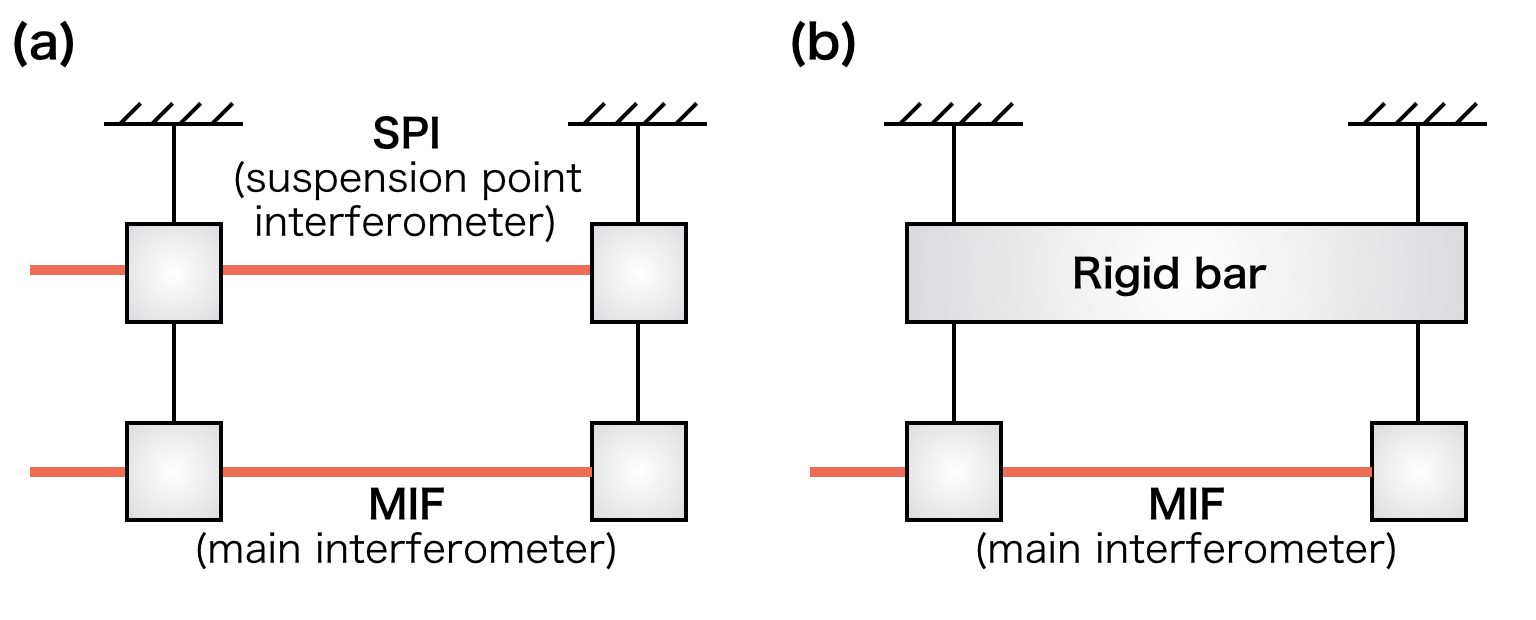
\includegraphics[width=13cm]{./img_chap5/img508.png}
    \caption{Schematic arrangement for one arm of SPI.} \label{img:img508}
  \end{center}
\end{figure}
Initial type of the SPI is, as shown in Figure \ref{img:img508}, the Fabry-perot optical cavity on the main interferometer's arm cavity \cite{drever2002extension}. The advantage of this idea is that this sytem can suppress the baseline length fluctuation using the feedback control because the SPI is installed near the main interferometer. Thus, if we increase the feedback gain, the length of the SPI behaves as the rigid bar as shown in Figure \ref{img:img508}(b). This means that the main cavity is suspended by the single pendulum from the ground, which does not change the baseline length entirely. Soon, 2 m proto type of SPI was developed and demonstrated about 40 db of vibration attenuation below 1 Hz \cite{aso2004stabilization}.

In general, the disadvantage of SPI is the noise coupling from the common motion due to the worse common mode rejection (CMR) above the eigenfrequency of the pendulums, because the active baseline vibration isolation system cannot attenuate the common motion of the baseline. If the mechanical response of the pendulums suspended from SPI stage have asymmetricity, the CMR is worse and the common motion couples to the baseline length change, which is the differential motion of the baseline.

The Fabry-Perot tyep SPI has problems in the km-scale GW detectors. While the displacement measurement of the Fabry-Perot cavity is precise, the linear range of the optical cavity is narrow (a few nm). Due to small dynamic range, the operation of the SPI becames unstable. As described in the section \cref{sec:sec313}, although the differential motion of short baseline is reduced efficiently, that of km-scale baseline is not reduced sufficiently. The reduction of km-scale baseline is a orders of threee greater than that of a few meter scale. Moreover, the alignment control is also difficult in the km-scale detectors.

\subsubsection{Michelson Interferometer Type}
%% \begin{figure}[h]
%%   \begin{center}   
%%     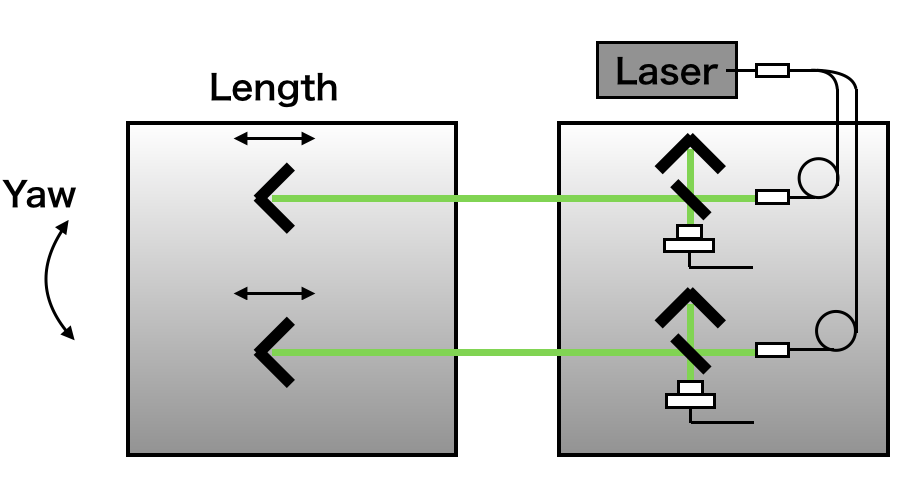
\includegraphics[width=9cm]{./img_chap5/img508a.png}
%%     \caption{Active baseline seismic isolation system using Michelson Type SPI \cite{Numata2008interferometric}. 2つのSPIで基線方向とYaw方向の制御をしている。それぞれのSPIはエンド鏡にコーナーキューブを使用している非対称マイケルソン干渉計であり、干渉信号はホモダイン検波で取得している\cite{araya2002iodine}。コーナーキューブは干渉させるためのアラインメント調整を必要としないが、その反面、角度変化と基線変化を区別できないので、SPIが2台必要になる。} \label{img:img508a}
%%   \end{center}
%% \end{figure}
To resolve the narrow linear range of the Fabry-Perot type SPI, a proto type of the Michelson type SPI was developed \cite{Numata2008interferometric}. The interferometer configuration of this proto type was the same as the GIF interferometer, and the signal detecton also the same. Thus, the type had the wide dynamic range wihout alignment control to keep the operation of the SPI. The proto type demonstrate the vibration supression of 2m baseline over several hours.

\subsection{Limitation due to CMRR}\label{sec532}
\begin{figure}[h]
  \begin{minipage}[t]{0.5\hsize}
    \centering
    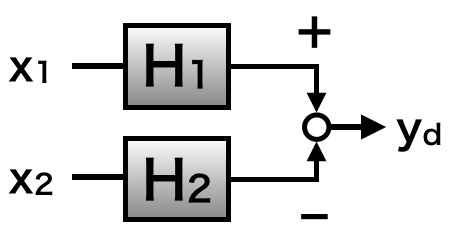
\includegraphics[width=6cm]{./img_chap5/img510a.png}
    \subcaption{two ground motion inputs ($x_1$ and $x_2$) one differential baseline change output ($y_{\mathrm{d}}$)} \label{img:img510a}
  \end{minipage}
  \begin{minipage}[t]{0.5\hsize}
    \centering
    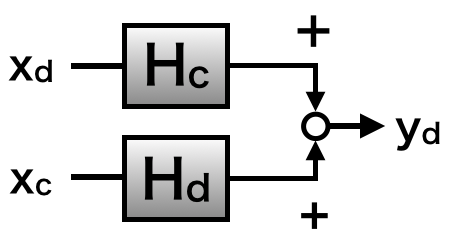
\includegraphics[width=6cm]{./img_chap5/img510b.png}
    \subcaption{two differential and common ground motion inputs ($x_{\mathrm{d}}$ and $x_{\mathrm{c}}$) one differential baseline change output ($y_{\mathrm{d}}$)} \label{img:img510b}
  \end{minipage}
  \caption{comparison of two representations.}
\end{figure}

While the active inertial seismic isolation described in the section \cref{sec:512}, the active baseline seismic isolation cannot isolate the common motion. Thus, if worse common mode rejection (CMR) of the suspensions, the common ground motion couples to the differential ground motion, which is the baseline length changes.


Consider the differential motion of the platform stages. As shown in Figure \ref{img:img510a}, the motion can be represented as 
\begin{eqnarray}
  y_{\mathrm{d}} = H_1x_1-H_2x_2 \label{eq:eq517},
\end{eqnarray}
where $x_{i},\,y_{d}$ and $H_{i}$ denote the ground motion, the stage motion, and the mechhanical transferfunction from the ground motion to the stage motion, respectively. The indicies of $i$ run in 1 or 2, which denote the name of the stages. Here, we define the differential and common motion of the ground and transferfunction as 
\begin{eqnarray} \label{eq:eq517_b}
  x_{\mathrm{d}} = {x_1-x_2},\ x_{\mathrm{c}} = {x_1+x_2}  \\
  H_{\mathrm{d}} = \frac{H_1-H_2}{2},\ H_{\mathrm{c}} = \frac{H_1+H_2}{2} \label{eq:eq517_a}.
\end{eqnarray}
The Eq(\ref{eq:eq517}) can be represented as 
\begin{eqnarray}
  y_{\mathrm{d}} &=& H_1x_1-H_2x_2 \\
  &=& H_{\mathrm{c}}x_{\mathrm{d}} + H_{\mathrm{d}}x_{\mathrm{c}}\label{eq:eq516}.
\end{eqnarray}
The last equation can be represented as shown in Figure \ref{img:img510b}. Moreover, if we define the CDMRR of this system as
\begin{eqnarray}
  H_{\mathrm{CMRR}} \equiv \frac{H_1+H_2}{H_1-H_2}=\frac{H_{\mathrm{c}}}{H_{\mathrm{d}}} \label{eq:eq519},
\end{eqnarray}
the differential system can be written as 
\begin{eqnarray}
  y_{\mathrm{d}} = H_{\mathrm{c}}\left( x_{\mathrm{d}} + \frac{1}{H_{\mathrm{CMRR}}}x_{\mathrm{c}}\right) \label{eq:eq518}
\end{eqnarray}
Eq.(\ref{eq:eq518}) indicates that increaseing the CMRR, the coupling from the common ground motion to the differential stage motion. In other words, the inverse of the CMRR is the coupling coefficient.

According to the definition of The CMRR, this factor is sensitive to the differential of two mechanical response. Thus, if the eigenfrequecy of each pendulum, the CMRR is worse above the frequency. For example, assume that the mechanical response of the stage is the single pendulum, which transfer function from the ground to stage can be given by Eq.(\ref{eq:eq502}). In the high frequency, above the eigen frequency, the response can be approximate as $H\sim{({f_0}/{f})^2}$. In this frequency region, if the eigen frequency shifts by $\Delta{f_0}$, the gain of the response differs by $2f_0\Delta{f_0}$. This amount worse the CMRR, and the common motion contaminates the differential motion.


\subsection{RMS Reduction}
The reduction of Root-mean-square (RMS) of the differential stage motion is expected by utilizing the SPI on the active seismic isolation system. Because the SPI has a good sensitivity in low-frequency including the microseisms and earth tides, the RMS of the differential stage motion can be reduced.

The reduction has some advantage for GW detectors.

\subsubsection{Improvement of Actuator Noise}
The RMS reduction of the differential stage motion can relax the requirement of the actuator on the test mass. The actuator on the test mass can only actuate weak force because the strong actuator would introduce the actuation noise to the sensitivity \cite{michimura2017mirror}. Therefore, the RMS reduction on the top stage can reduce the load on the test mass actuators. This means the improvement of the test mass actuator's noise directly, moreoever, means that the actuator's dynamic range can be became wider.

\subsubsection{Improvement of Glitch Noise}
The reduction of the test mass actuator's load reduce the glicth noise such as the Barkhausen noise. This noise is caused by the large DC voltage on the test mass actuators and actuators above the test mass \cite{aasi2015characterization}.




\section{Baseline Compensation System}\label{sec:52}
The baseline compensation system is the active baseline seismic isolation system uging the GIF. 

\subsection{Purpose}
The purpose of the baseline compensation system is to reduce the RMS of the cavity length fluctuation from 1 Hz to DC. In this region, the RMS motion in cavity length is mainly disturbed by the seismic noise such as the microseisms ($\sim 200\,\mathrm{mHz}$), large earthquake in distant place ($< 100\,\mathrm{mHz}$), air pressure response ($< 20\, \mathrm{mHz}$), and earth tides ($\sim 10^{-5}\,\mathrm{Hz}$). Moreover, the RMS of these seismic motion is comparable with several $1\sim100\,\mathrm{um}$, which is much greter than the test mass actuator's range. Therefore, the compensation of the cavity length disturbed by these seismic noise not only the improve stability of the detector operation but also the reduce the glitch noises in GW signal.

\subsection{Concept}
The concept of the baseline compensation system is the feedforward control, which move the platform stage at X-end using the baseline length changes measured by the GIF in order to compensate the seismic disturbance as shown in Figure \ref{img:img512}. The cavity's mirrors are suspended by the pendulums, whose suspension point is fixed on the platform stage. This platform stages is also suspended by the inverted pendulums on the second fllor. The platfrom responds the seismic motion below 1 Hz, which is the target frequency to be reuced. Thus the seismic disturbance of the stage motion is attenuated by using the actuator on the stage. The control signal is given by the GIF on the fisrt floor.
\begin{figure}[h]
  \begin{center}   
    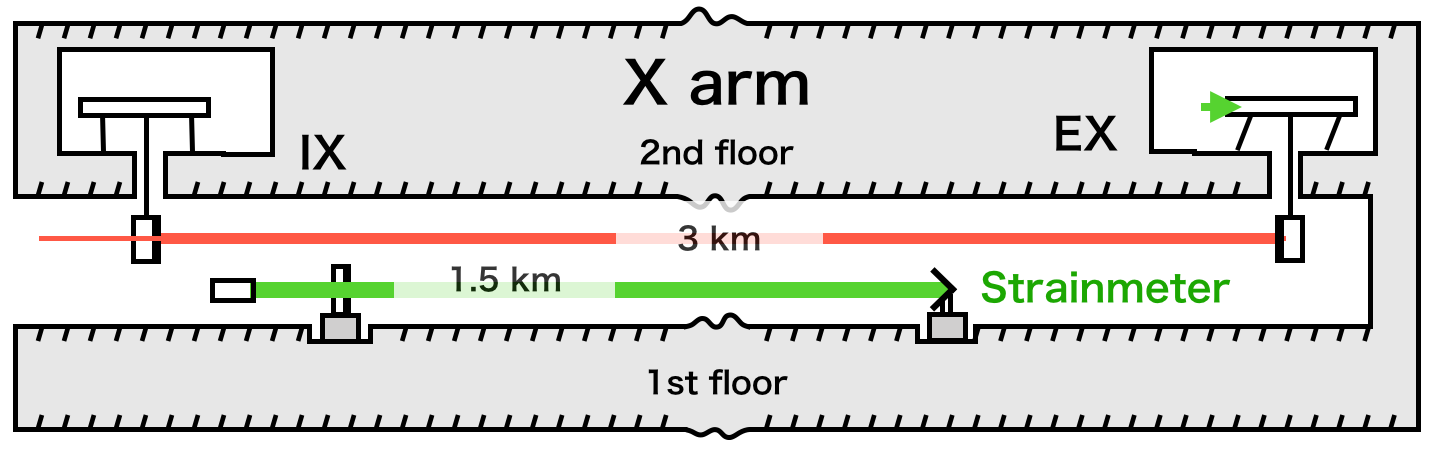
\includegraphics[width=14cm]{./img_chap5/img512.png}
    \caption{} \label{img:img512}
  \end{center}
\end{figure}

\subsection{GIF as a SPI}
The idea of this baseline compensation system is originate from the \cite{Numata2008interferometric} as mentiond in the section \ref{sec:321}. While this system used feedbac control, our system use feedforward control. The feedback control style baseline compensation system has some difficulty in terms of developing the km-scale system, because we need install the SPI, which measure the baseline length should be installed on the platform stage. This means that, in KAGRA case, additional tunnel is needed on the second floor to connect the platform stages. On the other hand, the feedforward style system does not need such facility, just reqiures the SPI, which can measure the baseline length in the tagert frequency, which is below 1 Hz.

In terms of the low-frequency, difference between the length change of 1500 m baseline and that of 3000 m baseline is differd by factor 2, according to Figure \ref{img:img411_a}.

\subsection{Control methods} \label{sec:444}
\begin{figure}[h]
  \begin{center}   
    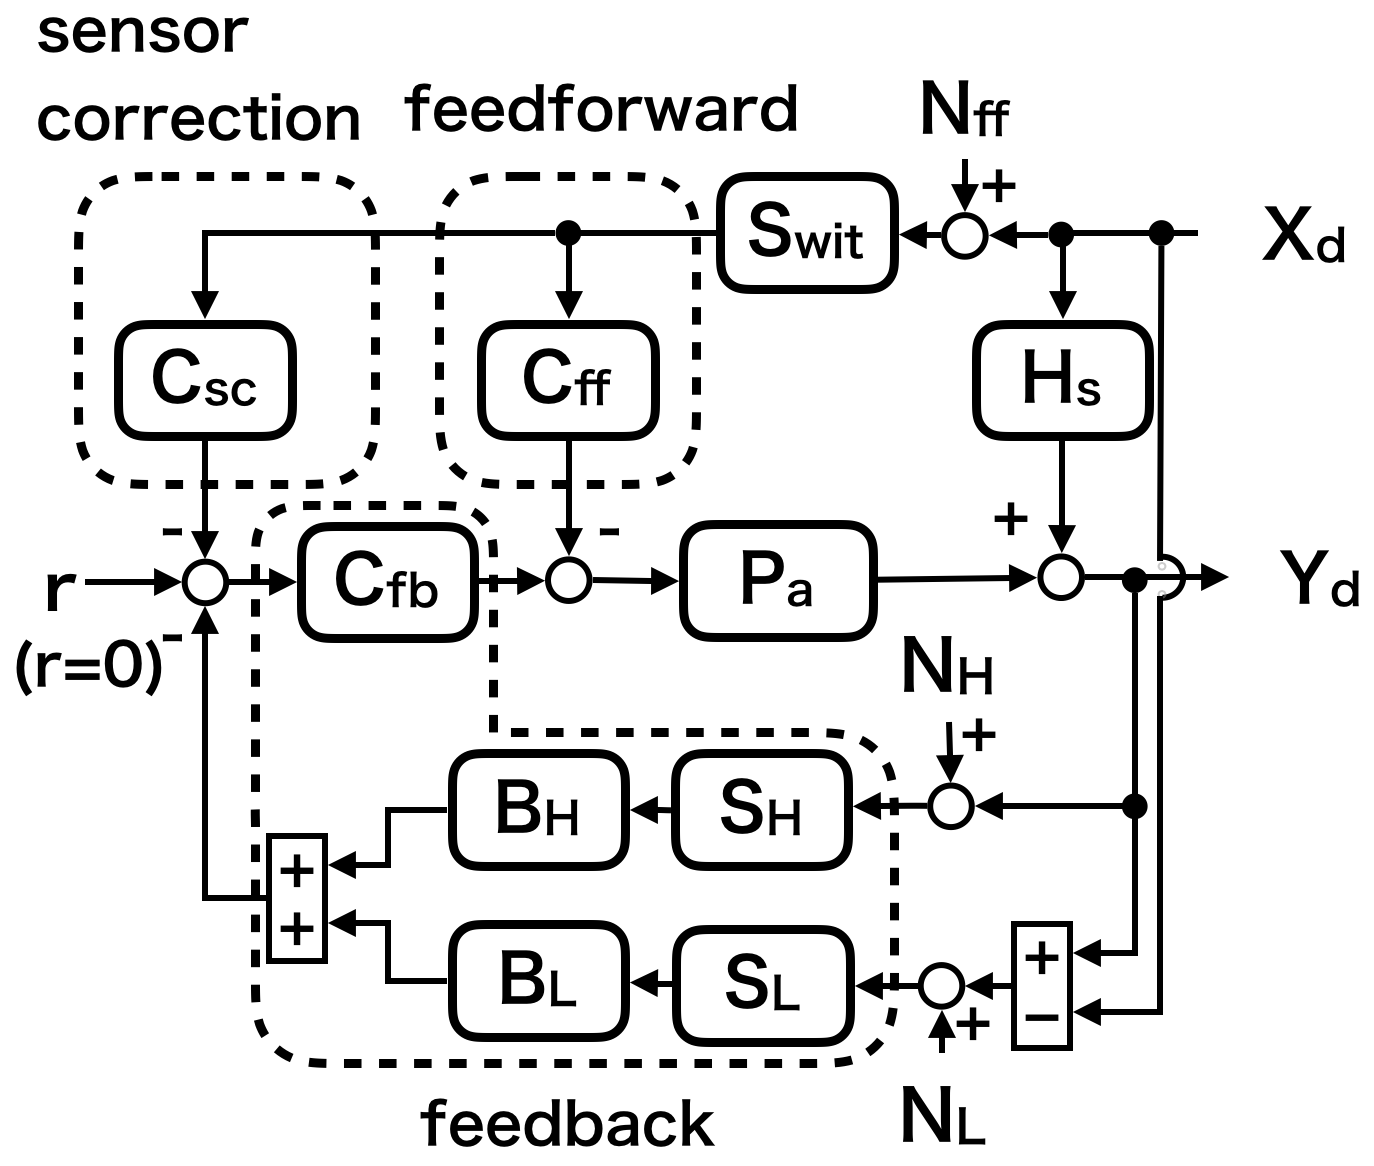
\includegraphics[width=10cm]{./img_chap5/img511.png}
    \caption{The block diagram of the active baseline seismic isolation system.} \label{img:img511}
  \end{center}
\end{figure}
We describe the general control scheme of the active baseline seismic isolation system using the feedforward type SPI. In this case, because of no feedback tyep SPI, the baseline length is controled by using the inertial sensor and relative position sensor as well as the active inertial iolation system. However, the additional control schemes such as the sensor correction and the feedforward are implimented in this new system.

The baseline isolation system attenuates, of course, the cavity length fluctuation. This fluctuation is the differential component of the displacement of the each test mass. To simplify the discussion, we supposed the CMRR is large enough to ignore the common motion coupling. Thus, we can just consider about the only differential component of the motion in this system.

The control diagram of the active baseline isolation system can be represented as shown in Figure \ref{img:img503}. Essentialy, all the terms in this figure is the same as the active inertial isolation system shown in Figure \ref{img:img503} except the input and output signals. There signals are replaced as $X_{\mathrm{d}}$ and $Y_{\mathrm{d}}$, which are the differential displacement of the ground and platform stage motions, resplectively. In this figure,  $S_{\mathrm{wit}}$ and $N_{\mathrm{ff}}$ are the frequency response and the selfnoise of the GIF, respectively. Furthermore, the noises $N_{\mathrm{H}}$ and $N_{\mathrm{L}}$ are multiplied by $\sqrt{2}$ in the case of the amplitude unit.

The displacement of the differential motion of the stages is given by 
\begin{eqnarray}\nonumber
  Y_{\mathrm{d}} &=&\frac{G}{1+G}L\Delta_{\mathrm{sc}} X_{\mathrm{d}} + \frac{1}{1+G} \Delta_{\mathrm{ff}} X_{\mathrm{d}}\\ \nonumber
  &+& \frac{G}{1+G}\left(HN_{H}+LN_{L}\right) + \frac{G}{1+G}C_{\mathrm{sc}}S_{\mathrm{wit}}N_{\mathrm{ff}} \\ 
  &+& \frac{1}{1+G}P_{\mathrm{a}} C_{\mathrm{ff}}S_{\mathrm{wit}}N_{\mathrm{ff}} \label{eq:eq520}.
\end{eqnarray}
As described about the active inertial seismic isolation system in section \ref{sec512}, both the additional reduction factors $\Delta_{\mathrm{sc}}$ and $\Delta_{\mathrm{sc}}$ can isolate the differential ground motion $X_{\mathrm{d}}$. Although the witness sensor was the inertial sensor in the previous iolation system, the new isolation system use the GIF, which can measure the seismic noise below 1 Hz and to DC. This is the advantage.

\section{Summary of the Chapter}
In this chapter, the following items are described:
\begin{itemize}
\item While the passive isolation system could isolate the seismic noise above its eigen frequency, which is tipicaly around 1 Hz, the active isolation systems are needed to compensate the low-frequency seismic noise below 1 Hz by isolating the platform stage from the seismic noise.
\item Two active isolation systems are described; the active {\it inertial} seismic isolation system attenuates the platform stages to the inertial frame, the active {\it baseline} seismic isolation system isolates the optical arm cavity's length from the deformation of the baseline.
\item The performance of the active inertial seismic isolation system is limited by the insufficient sensitivity and the tilt-holizontal coupling of the inertial sensor below 100 mHz.
\item Although the active baseline seismic ioslation is an effective method, the SPI which is the cavity length monitor has a difficulties in the longer scale GW detector.
\item The baseline compensation system using the GIF strainmeter resolve these limitaions and problems because the strainmeter can measure the deformation of the baseline below 1 Hz without tilt-coupling and the strainmeter can observe the baseline fluctuation independent from independent of the GW detector.
\end{itemize}
